\hypertarget{kyoto-autour-de-kyoto-et-hiroshima.}{%
\section{Kyoto, autour de Kyoto et
Hiroshima.}\label{kyoto-autour-de-kyoto-et-hiroshima.}}

Nous avons quitté Tokyo avec le Shinkansen. Ce train rapide, symbole
international du Japon, se distingue par ses retards incroyablement
faibles qui se comptent en moyenne \emph{en dizaines de seconde par
train}, tous trajets cumulés sur une année. Bien sûr, il faut préciser
que ce train rapide est également très cher (environ 110 euros pour 450
kilomètres en deux heures et demi pour un Tokyo - Kyoto).

Manque de chance, des pluies exceptionnelles ont perturbé le service
lors de notre trajet vers Kyoto. C'est donc avec plus de deux heures de
retard que nous arrivons à destination. En plus de dix ans de séjours au
Japon, je sais que c'est exceptionnel. Et malheureusement ces
inondations ont fait des victimes nombreuses dans l'ouest du Japon.
Pourtant, à Kyoto, la situation est sous contrôle. Mis à part la rivière
Kamo qui est en crue, nous ne détectons rien de particulier. D'ailleurs,
la chaleur est étouffante. La température est systématiquement au-dessus
de 30 degrés, l'air humide. Ce qui n'a pas empêché la pluie de nous
surprendre plus d'une fois.

\begin{figure}
\centering
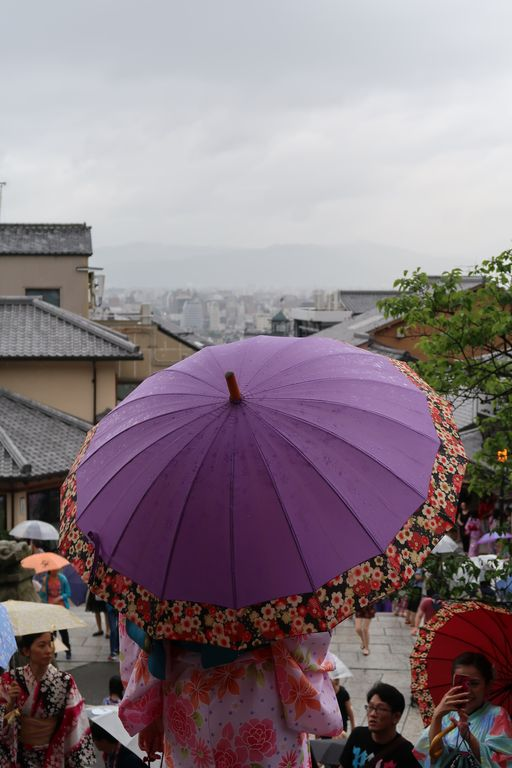
\includegraphics{images/20180716_kyoto.JPG}
\caption{Ambiance parapluie à Kyoto.}
\end{figure}

Nous retiendrons de Kyoto son ambiance à la fois rustique et branchée,
notamment entre Kawaramachi et Shijo, une rivière Kamogawa en crue ou
encore l'allure traditionnelle du quartier autour du Kiyomizudera (et
ses nombreux touristes), le temple de l'eau pure. Et le karaoké, qui
nous a donné l'occasion de chanter du Céline Dion par temps de pluie.

Cela dit, notre coup de coeur va à Arashiyama. A quelques dizaines de
minutes à l'ouest du centre de Kyoto, ce quartier à flanc de montagne
nous a fait découvrir de très beaux jardins et l'étonnante forêt des
singes. On peut y observer une tribu de macaques japonais de très près
(moment mignonitude devant les bébés) tout en profitant du cadre
idyllique.

\begin{figure}
\centering
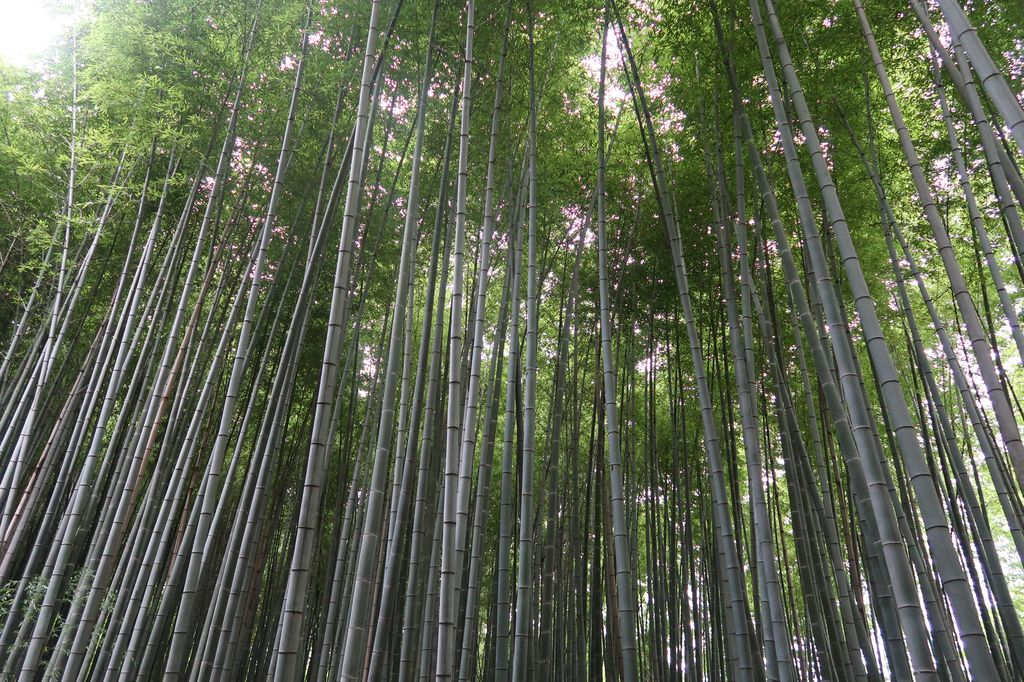
\includegraphics{images/20180716_bambou.JPG}
\caption{Les spectaculaires bambous d'Arashiyama.}
\end{figure}

Notre plus beau coucher de soleil, ce fut au sommet du mont Inari auquel
on grimpe par l'intermédiaire du sanctuaire Fushimi Inari, le fameux
sanctuaire aux dix-mille portes Torii.

\begin{figure}
\centering
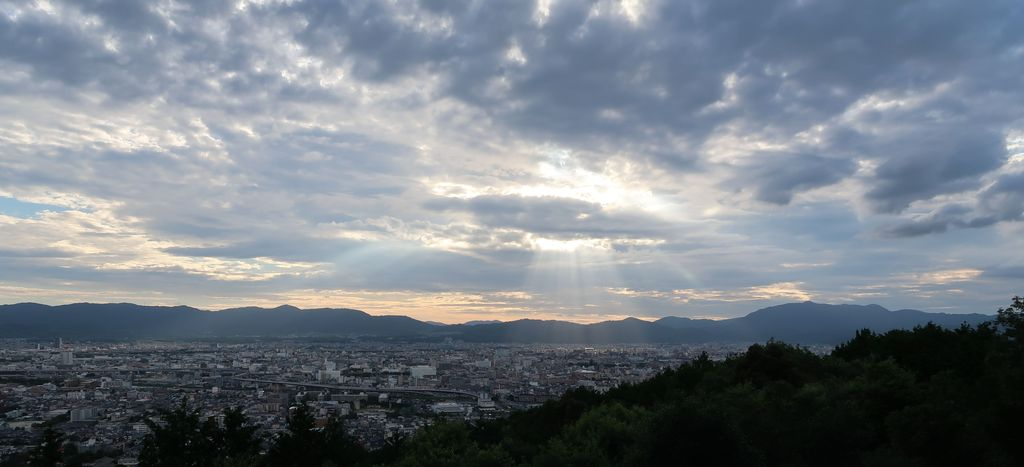
\includegraphics{images/20180716_inari.JPG}
\caption{Kyoto, vue de l'ouest.}
\end{figure}

Nous avons également profité du passage à Kyoto pour aller à Hiroshima,
à la faveur d'un lever aux aurores et du Shinkansen (de nouveau tout à
fait opérationnel). Nous y avons rendu visite à l'île de Miyajima (et y
voir une séance photo de mariage dans le sanctuaire local), vu un
célèbre Torii, mangé un okonomiyaki. On a fini par le mémorial de
l'attaque nucléaire de 1945. Pour nous remonter le moral après cette
triste visite, un petit MacDo à grande vitesse sur le chemin du retour
n'était pas de trop.

\begin{figure}
\centering
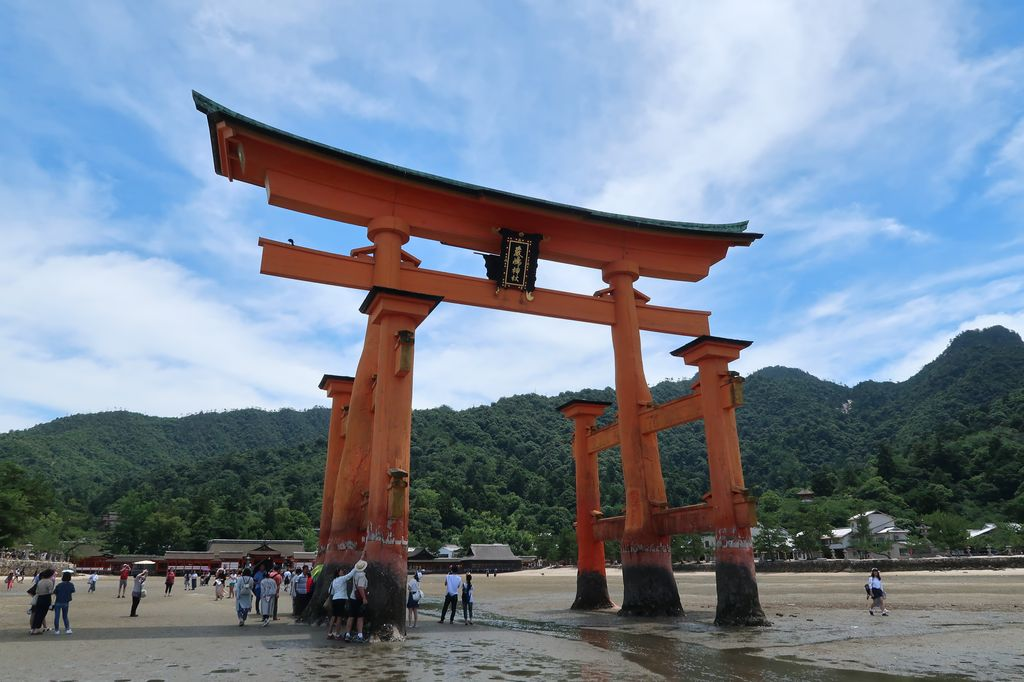
\includegraphics{images/20180716_torii.JPG}
\caption{Le Torii "les pieds dans l'eau" de Miyajima, au large
d'Hiroshima.}
\end{figure}

Pour finir, laissez-moi vous raconter comment on prend le bus à Kyoto
(et préparez vous à un sacré contraste avec la France) :

\begin{itemize}
\tightlist
\item
  on entre dans le bus par la porte arrière (et on sortira par celle de
  devant)
\item
  la tarification du trajet est soit un tarif unique, soit fonction de
  la distance, auquel cas cette distance est "mesurée" à l'aide d'un
  petit ticket papier que l'on prend en entrant et sur lequel est
  inscrit le numéro de la station initiale ; un écran informe ensuite
  les passagers des tarifs pour les différents points de départ
\item
  on cherche un endroit où s'asseoir
\item
  on s'étonne que le trajet soit commenté en direct par le chauffeur de
  bus, par exemple : "attention, virage en vue", "désolé, on doit
  s'arrêter au feu rouge", "c'est reparti !", ce qui anime le trajet !
\item
  une fois la destination en vue, on anticipe la descente et on se
  dirige vers la porte avant du bus
\item
  on prépare le montant exact demandé afin de le mettre dans une petite
  boîte à gauche du chauffeur
\item
  si l'on n'a pas pile la monnaie, on utilise la machine qui permet de
  faire du change (par exemple transformer un billet de 1000 yens en
  pièces de 500, 100 et 10 yens)
\item
  enfin, le chauffeur nous gratifie d'un \emph{arigato gozaimasu} bien
  senti lors du paiement et de la descente
\end{itemize}

Alors, ça donne pas envie de prendre le bus au Japon \^{}\^{} ?

\emph{Florian et Elida}
